\documentclass[a4paper,12pt]{article}
\usepackage[MeX]{polski}
\usepackage[utf8]{inputenc}
\usepackage{graphicx}


%opening
\title{}
\author{}

\begin{document}

\maketitle

\section {Drugi gabinet Bena Chifleya(ang. Second Chifley Ministry)} trzydziesty czwarty gabinet federalny Australii, urzędujacy od 1 listopada 1946 do 19 grudnia 1949 roku. Byl piatym z rzędu jednopartyjnym gabinetem tworzonym przez Australijską Partię Pracy (ALP) i zarazem ostatnim lewicowym gabinetem przed dwudziestotrzyletnia przerwa, w czasie której ALP pozostawala cały czas w opozycji.

\section {Okolicznosci powstania i dymisji}

Gabinet urzędował przez cala trzyletnia kadencje Izby Reprezentantow. Jego powstanie było konsekwencja wyborow parlamentarnych z wrzesnia 1946, w ktorych ALP obronila pozycje partii rzadzacej, zas Ben Chifley stanowisko premiera. Zarazem polityk ten po raz pierwszy (i ostatni) uzyskał demokratyczną legitymację jako szef rządu, jako że w 1945 objął to stanowisko w środku kadencji na mocy decyzji samej partii, której członkowie wybrali go na nowego lidera w miejsce zmarłego Johna Curtina.

Kolejne wybory odbyły się w grudniu 1949 i przyniosły zwycięstwo ALP tylko w Senacie. W Izbie Reprezentantów, mającej decydujące znaczenie dla obsady stanowiska premiera, wygrała opozycyjna Koalicja, zaś jej lider, Robert Menzies, powrócił do kierowania rządem po ponad ośmioletniej przerwie i utworzył swój czwarty gabinet.

\begin{table}
\begin{tabular}{lccc}
\hline
\textbf{stanowisko}&\textbf{osoba}&\textbf{od}&\textbf{do}\\
\hline
premier&Ben Chilfley&1 listopada 1946 & 19 grudnia 1949\\
minister skarbu&Ben Chifley&1 listopada 1946&19 grudnia 1949\\
minister obrony&John Dedman&1 listopada 1946&19 grudnia 1949\\
minister sił powietrznych&Arthur Drakeford&1 listopada 1946&19 grudnia 1949\\
minister imigracji&Arthur Calwell&1 listopada 1946&19 grudnia 1949\\
minister zaopatrzenia rozwoju&John Armstrong&6 kwietnia 1948&19 grudnia 1949\\
\hline
\end{tabular}
\caption{Sklad}
\end{table}


\section {Bibliografia}
\begin{itemize}
\item 43rd Parliamentary Handbook (ang.). Parliament of Australia. [dostęp 2014-02-05].
\item Ben Chifley (ang.). National Archives of Australia. [dostęp 2014-02-05].
\end{itemize}

\begin{figure}
\centering
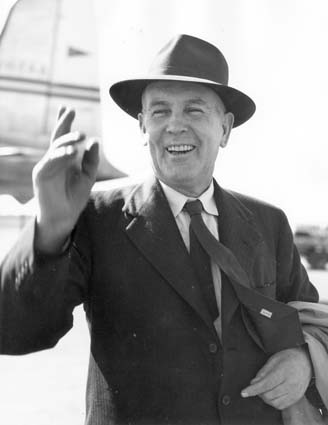
\includegraphics[width=10cm]{BenChifley.jpg}
\caption{Ben Chilfley}
\label{BenChifley.jpg}
\end{figure}


%https://pl.wikipedia.org/wiki/Drugi_gabinet_Bena_Chifleya
%https://pl.wikipedia.org/wiki/Lasocin_(wojew%C3%B3dztwo_dolno%C5%9Bl%C4%85skie)

\end{document}